%% Applied Intelligence submission — Springer Nature template (sn-jnl)
%% Build: latexmk -pdf main.tex
\documentclass[pdflatex,sn-basic]{sn-jnl}

\usepackage{amsmath,amssymb}
\usepackage{xcolor}
\usepackage{graphicx}
\usepackage{booktabs}
\usepackage{array}

\begin{document}

\title[Sequential Hybrid Sampling for Imbalanced DTI Prediction]{Sequential Hybrid Sampling with Informed Undersampling for Imbalanced Drug--Target Interaction Prediction}

\author*[1]{\fnm{Isman} \sur{Kurniawan}}\email{ismankrn@telkomuniversity.ac.id}
\author[2]{\fnm{Rizky Nurhaliza} \sur{Harahap}}\email{rizky\_harahap@aprilasia.com}
\author[1]{\fnm{Fhira} \sur{Nhita}}\email{fhiranhita@telkomuniversity.ac.id}
\author[3]{\fnm{Afizan} \sur{Azman}}\email{afizan.azman@taylors.edu.my}

\affil*[1]{\orgdiv{School of Computing}, \orgname{Telkom University}, \orgaddress{\city{Bandung}, \country{Indonesia}}}
\affil[2]{\orgname{Asia Pacific Resources International Holdings Limited (APRIL)}, \orgaddress{\city{Pangkalan Kerinci}, \state{Riau}, \country{Indonesia}}}
\affil[3]{\orgname{Taylor's University}, \orgaddress{\street{1, Jln Taylors}, \postcode{47500} \city{Subang Jaya}, \state{Selangor}, \country{Malaysia}}}

\abstract{Drug--target interaction (DTI) datasets are extremely imbalanced, and
resampling is the standard remedy. However, many resampling studies in
this field rely on a single train--test split without statistical
testing. We evaluated the sequential hybrid sampling (SHS) framework, in
which the minority class is oversampled beyond the majority size and an
undersampling stage then selects the balancing subset, with ant colony
optimization (ACO) and simulated annealing (SA) as informed
selectors and random selection as the control. Thirteen methods were compared on four gold-standard Yamanishi datasets under a repeated
multi-seed protocol with paired statistical tests, with a full factorial ablation of the ACO undersampler and a budget-matched SA
comparator. To our knowledge, this is the first systematic evaluation of
the overproduce-and-choose resampling paradigm in DTI prediction. A
single split proved unreliable, in which the F1 score of one
configuration ranged from 0.267 to 0.431 across splits. The ACO undersampler was robust to its
implementation details, and the budget-matched SA was statistically
indistinguishable from it, so that the value lies in informed selection
rather than in a particular metaheuristic. The winning oversampler shifts from ROS to SMOTE and
ADASYN as the minority grows, resampling lifts the best F1 from 0.32
to 0.47 on the smallest dataset, and no method beats the baseline
on the richest one, where ACO abstained in all runs,
acting as a safety valve. Informed selection costs up to about 460 times more than random selection and pays off mainly under extreme
scarcity. Code, data, and results are publicly available.}

\keywords{drug--target interaction, class imbalance, hybrid sampling, informed undersampling, ant colony optimization, simulated annealing}

\maketitle

\section{Introduction}

A drug--target interaction (DTI) is the binding of a drug to a
selective target site that modifies the function or behavior of the
target \citep{azlimkhan2023comparative}. The drug is a chemical
compound that induces a physiological change once it enters the body,
while the target is a biological macromolecule, typically a protein,
that produces this change upon binding \citep{you2018drug}. Identifying
DTIs is therefore central to understanding the mechanism of action of a
drug, anticipating its side effects, and finding new uses for approved
compounds through drug repositioning \citep{bagherian2021machine,
azlimkhan2023comparative}. The main druggable target families are
enzymes, ion channels, G-protein-coupled receptors, and nuclear
receptors, and the gold-standard datasets compiled by
\citet{yamanishi2008prediction} for these four families serve as the
common benchmark for DTI prediction.

In the laboratory, DTIs are identified through experimental techniques
such as high-throughput screening and biochemical assays. These
techniques provide reliable evidence, yet they are time-consuming,
labor-intensive, and costly, while the space of candidate drug--protein
pairs is enormous \citep{you2018drug, barkat2021drug}. Computational
prediction is therefore widely used to prioritize candidate pairs before
laboratory testing. Among the computational approaches, feature-based
machine learning represents each drug--protein pair by chemical and
sequence descriptors and casts the prediction as binary classification
\citep{chen2018machine}, and recent pipelines such as SRX-DTI provide
standardized feature representations for the benchmark datasets
\citep{khojasteh2023improving}.

These datasets have two inconvenient properties. First, the negatives
are unverified, since the pairs that are not listed in the gold standard
are merely unlabeled \citep{shi2019predicting}. Second, the class
distribution is extremely imbalanced, in which the positive rate ranges
from approximately 6\% down to below 1\%. Under such imbalance, a
classifier that favors the majority class attains a high accuracy while
missing most of the interactions, so that the minority performance has
to be measured by metrics such as F1, G-Mean, and the area under the
precision--recall curve \citep{saito2015precision}. Resampling has
therefore become a standard companion of DTI classifiers, e.g.,
SMOTE-based oversampling in iDTi-CSsmoteB \citep{mahmud2019idti}, class
balancing combined with feature selection \citep{redkar2020machine},
and comparative studies of resampling techniques for DTI models
\citep{azlimkhan2023comparative}.

Remedies for class imbalance operate at two levels. Algorithm-level
approaches modify the learner itself, e.g., through cost-sensitive
losses, decision-threshold adjustment, or ensemble schemes, while
data-level approaches modify the training distribution before any
learner is applied \citep{mohammed2020machine, devi2020review}. The
data-level route is attractive in practice because it is
classifier-agnostic, in which the same balanced training set can feed
any downstream model, and because its effect can be examined
independently of the learner \citep{kim2022empirical}. For these
reasons, data-level resampling has become the dominant route in DTI
prediction.

Resampling-based DTI prediction has advanced considerably on this
benchmark. \citet{shi2019predicting} combined evolutionary and
chemical-structure features with Lasso dimension reduction, SMOTE, and a
random forest, and reported accuracies between 94.88\% on NR and
98.09\% on Enzyme. \citet{mahmud2019idti} paired SMOTE with XGBoost in
iDTi-CSsmoteB and obtained average auROC values between 0.9459 on NR and
0.9860 on Enzyme. \citet{redkar2020machine} combined wrapper feature
selection with SMOTE and several classifiers, and achieved accuracies
between 90.6\% and 95.9\% on the same four datasets after 10-fold
cross-validation. More recently, \citet{azlimkhan2023comparative}
compared resampling techniques across machine learning and deep learning
DTI models and confirmed that the choice of the resampling technique
materially affects the predictive performance.

In parallel, the resampling methods themselves have evolved. Random
over- and undersampling were followed by SMOTE, which interpolates
between minority neighbours \citep{chawla2002smote}, by the hybrid
SMOTE-ENN and SMOTE-Tomek methods, which clean the oversampled data by
using edited nearest neighbours or Tomek links \citep{batista2004study},
and by ADASYN, which concentrates the synthesis on the minority samples
that are harder to learn \citep{he2008adasyn}. The behavior of this
family has been studied extensively \citep{fernandez2018smote,
kim2022empirical, wongvorachan2023comparison, mohammed2020machine,
devi2020review}. A younger line treats the choice of the retained
instances as a search problem, in which ACOSampling selects majority
subsets by using an ant colony \citep{yu2013acosampling}, FF-SMOTE
tunes the synthetic values by using the firefly algorithm
\citep{kaur2019ffsmote}, and SAUS searches majority subsets by using
simulated annealing \citep{chennuru2022simulated}. Most recently, ESMOTE
introduced an overproduce-and-choose strategy on general benchmark data,
in which a large set of synthetic examples is generated first and an
evolutionary search then keeps the helpful ones \citep{zhang2023esmote}.
A sequential hybrid sampling (SHS) scheme follows the same paradigm, in
which the minority class is oversampled beyond the majority size to a
controlled pool ratio and an undersampling stage then selects the
exactly balancing subset by using a cross-validated objective. In
contrast to the rule-based cleaning of the classical hybrids, the
selection is informed by a global objective, a random selector can serve
as the uninformed control, and the selector may abstain when no subset
improves on the original data.

A two-stage framework of this kind opens a considerable design space.
The practitioner has to choose the oversampler that builds the pool, the
size of the pool relative to the majority class, the selector together
with its search budget, and the objective that drives the selection.
These choices interact, e.g., a larger pool offers more room to an
informed selector but merely more noise to a random one, and the search
budget directly multiplies the computational cost, since every candidate
subset is evaluated by cross-validation. In the existing
metaheuristic-sampling studies, these components are usually fixed in an
ad hoc manner and are rarely ablated, so that it is difficult to
attribute the reported gains to a specific component.

A closer look at this state of the art reveals four gaps. First, the
reported figures rely on accuracy or auROC, which remain optimistic
under extreme imbalance and can mask poor minority performance
\citep{saito2015precision}. On these datasets, an accuracy above 93\%
is attainable by always predicting the majority class. Second, each
study evaluates under a single protocol, in which one split or one
cross-validation round is used without statistical testing, so that the
stability of the conclusions is unknown. Third, the proposed resampling
methods are rarely compared head-to-head with the established hybrid
baselines under one common protocol. Fourth, the metaheuristic-selection
line, including the recent overproduce-and-choose strategy, was
developed largely outside DTI and has not been evaluated across the DTI
datasets, so that it is unclear whether its gains generalize and whether
they come from the specific algorithm or from informed selection in
general.

Addressing these gaps requires a particular evaluation design rather
than a new algorithm alone. The optimism of accuracy-based reporting can
be avoided by measuring the minority performance directly through F1,
G-Mean, balanced accuracy, and the area under the precision--recall
curve. The fragility of a single split can be exposed and controlled by
repeating every experiment over multiple random splits and by comparing
the methods with paired statistical tests. The missing baselines can be
restored by evaluating the classical oversamplers and the established
hybrids side by side with the metaheuristic variants under one common
protocol. The remaining uncertainty about the source of the gains can be
resolved by ablating the components of the search and by matching its
budget against an alternative metaheuristic and a random control.

Accordingly, the objective of this study is to establish when the SHS
framework with informed undersampling pays off in DTI prediction.
Specifically, this study aims to evaluate the generalization of the
framework across the four gold-standard datasets against the classical
and hybrid baselines, to examine the robustness of the ACO undersampler
to its implementation choices, parameters, and fitness function, and to
determine whether the benefit originates from informed selection itself
rather than from a particular metaheuristic.

The contributions of this study are as follows.
\begin{itemize}
  \item To our knowledge, the first systematic evaluation of the
        overproduce-and-choose resampling paradigm in DTI prediction,
        covering 13 methods on the four gold-standard datasets under a
        repeated, multi-seed protocol with paired statistical tests
        (725 runs in total).
  \item The identification and verification of the abstention property,
        in which the informed selector declines to resample when
        resampling is harmful, proposed here as an explicit design
        element for optimization-based resampling.
  \item A budget-matched SA comparator with a random-selection control,
        which shows that the value lies in informed selection itself
        rather than in the specific metaheuristic.
  \item A full factorial ablation of the ACO undersampler together with
        a parameter-sensitivity analysis, which shows that the method is
        robust to its implementation details.
  \item A practical map that matches the oversampler, the selector, and
        the pool ratio to the minority richness of the dataset, together
        with the associated computational costs.
  \item Publicly available code, data pipeline, and complete results.
\end{itemize}

% =========================================================================
\section{Materials and Methods}

\subsection{Datasets}
In this study, we used four gold-standard DTI datasets introduced by
\citet{yamanishi2008prediction}, i.e., nuclear receptor (NR),
G-protein-coupled receptor (GPCR), ion channel (IC), and enzyme (Enzyme)
datasets. Each dataset corresponds to a different class of target
protein. The features of drug--target pairs were generated by using the
SRX-DTI pipeline \citep{khojasteh2023improving}. Each drug was
represented by a 256-bit FP2 molecular fingerprint, while each protein
was represented by the amino acid composition (AAC, 20 features) and the
dipeptide composition (DPC, 400 features), resulting in 676 features per
pair. All feature columns were normalized by using min--max normalization
within each dataset. The instances were constructed from the full
Cartesian product of drugs and target proteins. The pairs listed in the
gold standard were labeled as positive, while the remaining pairs were
treated as negative. This assumption is standard in this field, although
the unlabeled pairs may contain undiscovered interactions. The statistics
of the four datasets are summarized in Table~\ref{tab:datasets}. The
positive rate ranges from 6.41\% in NR to 0.99\% in Enzyme, while the
number of real positive pairs in the training split increases from 63 in
NR to 2{,}048 in Enzyme. We refer to this gradient throughout the
Discussion. We did not apply any feature selection, so that the feature
representation is fixed and any performance difference is attributable
to the sampling strategies.

\begin{table}[htbp]
\centering
\caption{The statistics of the four gold-standard DTI datasets with the
stratified 70/30 split.}
\label{tab:datasets}
\setlength{\tabcolsep}{4pt}%
\footnotesize
\begin{tabular}{lccccccc}
\toprule
Dataset & Drugs & Targets & Pairs & Positives & Positive rate (\%) & Train positives & Test positives \\
\midrule
NR & 54 & 26 & 1,404 & 90 & 6.41 & 63 & 27 \\
GPCR & 223 & 95 & 21,185 & 635 & 3.00 & 444 & 191 \\
IC & 210 & 204 & 42,840 & 1,476 & 3.45 & 1,033 & 443 \\
Enzyme & 445 & 664 & 295,480 & 2,926 & 0.99 & 2,048 & 878 \\
\bottomrule
\end{tabular}
\end{table}

\subsection{Sequential hybrid sampling framework}
The sequential hybrid sampling (SHS) framework balances the training data
in two stages, as illustrated in Figure~\ref{fig:framework}. In the first
stage, the minority class was oversampled beyond the majority size to
produce a pool of synthetic candidates, in which the pool size was set to
$r \times n_{\text{maj}}$, where $r$ denotes the pool ratio and
$n_{\text{maj}}$ denotes the number of majority instances in the training
set. In the second stage, the pool was undersampled back to a balanced
size by selecting a subset of the candidates. This design differs from
classical hybrid methods such as SMOTE-ENN and SMOTE-Tomek
\citep{batista2004study}, which clean noisy instances after oversampling.
In contrast, SHS selects the subset of synthetic candidates by using an
optimization procedure. We considered three pool ratios, i.e., 1.0, 1.25,
and 1.5. A ratio-based formulation was adopted, rather than an absolute pool
size, so that the framework is portable across datasets. The ratio of 1.0 serves as a degenerate control, in
which the pool size is close to the required number of samples and the
selector has almost no choice. Three oversamplers were employed to build
the pool, i.e., random oversampling (ROS), SMOTE with $k=11$
\citep{chawla2002smote}, and ADASYN \citep{he2008adasyn}. Three selectors
were compared to perform the undersampling, i.e., random undersampling
(RUS) as an uninformed baseline, along with ant colony optimization (ACO)
and simulated annealing (SA) as informed selectors. Each combination is
denoted as SHS-\emph{selector} (\emph{oversampler}) in the remainder of
this paper.

\begin{figure}[htbp]
\centering
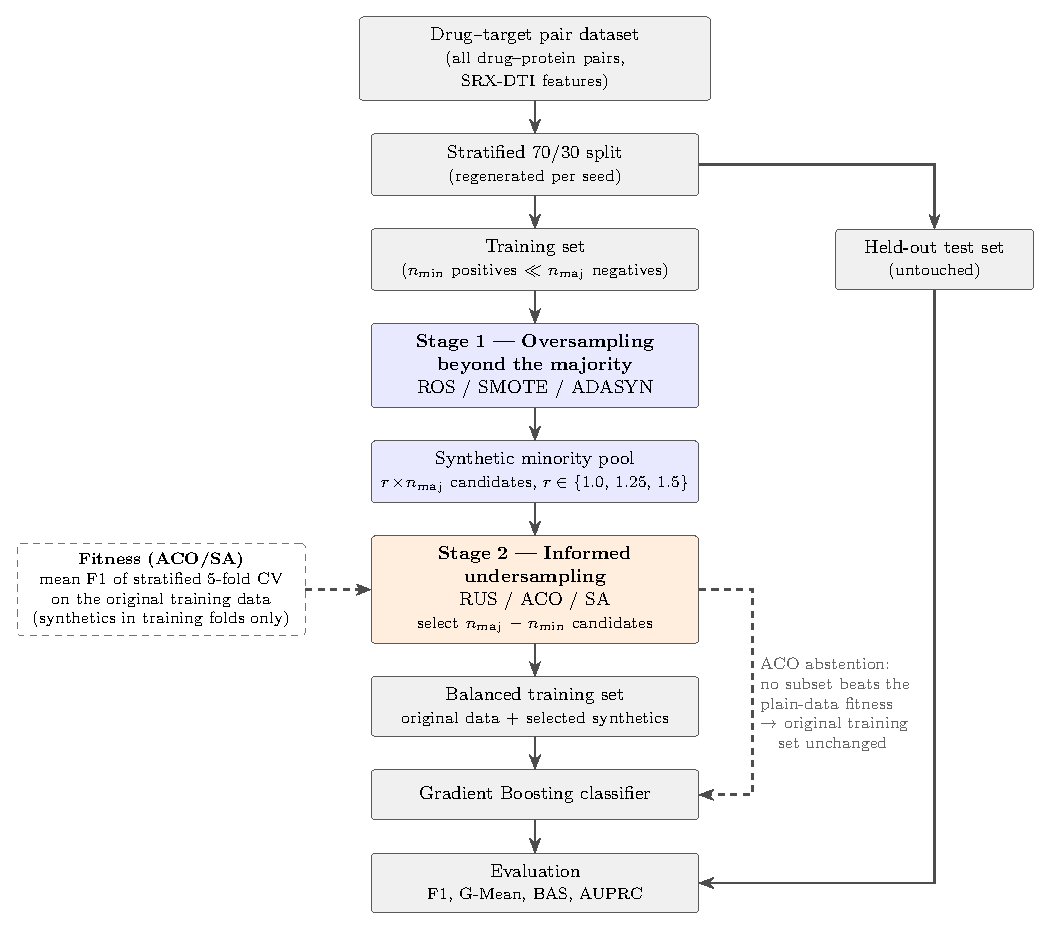
\includegraphics[width=0.78\textwidth]{Fig1.pdf}
\caption{The workflow of the sequential hybrid sampling framework}
\label{fig:framework}
\end{figure}

\subsection{ACO undersampler}
\label{sec:aco}
The ACO undersampler searches for the subset of synthetic candidates that
maximizes a cross-validated fitness \citep{dorigo2006ant,
yu2013acosampling}. The undersampling is formulated as a combinatorial
selection over the oversampled pool. A solution is represented as a
binary vector, analogous to a chromosome in evolutionary algorithms,
whose length equals the number of synthetic candidates in the pool. A
value of 1 indicates that the corresponding candidate is included in the
training data, while a value of 0 indicates that the candidate is
excluded. The core of the optimization is therefore to find the
combination of 1 and 0 values that yields the highest fitness. To ensure
that the minority size matches the majority size after the selection,
the number of 1 values is constrained to $n_{\mathrm{maj}} - n_{\min}$,
so that the selected candidates together with the $n_{\min}$ original
minority instances balance the $n_{\mathrm{maj}}$ majority instances.
This constraint is enforced by construction rather than by a penalty
term, in which each ant builds a solution by sampling exactly
$n_{\mathrm{maj}} - n_{\min}$ candidate indices from the pool. Since the
sampling was performed with replacement, a candidate may be selected
more than once, so that an entry of the solution vector may take an
integer count larger than 1. The effect of this choice was examined in
the ablation study (Section~\ref{sec:ablation}). Each of the $K$ ants
samples these candidate indices according to the selection probability
expressed as
\begin{equation}
  P_i = \frac{\tau_i}{\sum_{j} \tau_j},
  \label{eq:prob}
\end{equation}
where $\tau_i$ denotes the pheromone value of candidate $i$. The
pheromone values were initialized uniformly at $\tau_0 = 0.3$. After all
ants finish in one iteration, the pheromone values were updated by using
the standard rule expressed as
\begin{equation}
  \tau_i^{(t+1)} = (1-\rho)\,\tau_i^{(t)} + \Delta_i,
  \label{eq:pheromone}
\end{equation}
where $\rho$ denotes the evaporation rate and $\Delta_i$ denotes the
fitness accumulated over the ants that selected candidate $i$. The
quality of a solution was measured by the objective function expressed
as
\begin{equation}
  \max_{\mathbf{s}}\; f(\mathbf{s}) = \frac{1}{5}\sum_{k=1}^{5}
  \mathrm{F1}\!\left(h_{\mathbf{s}}^{(k)},\,
  \mathcal{D}_{\mathrm{val}}^{(k)}\right)
  \quad \text{subject to} \quad
  \sum_{i=1}^{M} s_i = n_{\mathrm{maj}} - n_{\min},
  \label{eq:objective}
\end{equation}
where $M$ denotes the pool size, $h_{\mathbf{s}}^{(k)}$ denotes the
classifier trained on the $k$-th training folds of the original training
data augmented with the candidates selected by $\mathbf{s}$, and
$\mathcal{D}_{\mathrm{val}}^{(k)}$ denotes the $k$-th validation fold.
The folds were stratified on the class label, and the synthetic
candidates were added to the training folds only. The solution
representation and the search cycle are illustrated in
Figure~\ref{fig:aco}. The search was run for $N = 10$ iterations, or $N = 5$ on Enzyme for feasibility (Section~\ref{sec:design}), with an early stop after five iterations without improvement. The evaporation rate was set to $\rho = 0.8$, and its sensitivity is
examined in Section~\ref{sec:ablation}, while the number of ants $K$ is
discussed in Section~\ref{sec:design}. The best
solution found across all iterations was returned as the final
selection. In addition, the implementation has an abstention property.
The fitness of the unmodified training data was evaluated as the initial
reference, and if no ant solution exceeds this reference, the
undersampler returns the original training data without any synthetic
candidates.

\begin{figure}[htbp]
\centering
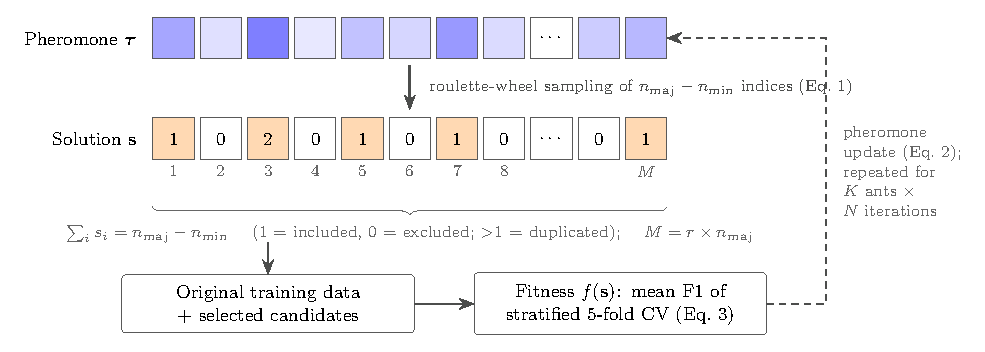
\includegraphics[width=0.95\textwidth]{Fig2.pdf}
\caption{The illustration of the ACO undersampler}
\label{fig:aco}
\end{figure}

\subsection{Budget-matched SA comparator}
\label{sec:sa}
To examine whether the benefit of informed selection is specific to ACO,
we compared it with simulated annealing (SA) as an alternative search
strategy \citep{kirkpatrick1983optimization, chennuru2022simulated}. SA
operates on the same solution space as the ACO undersampler, i.e., a
solution vector subject to the constraint in Eq.~(\ref{eq:objective}),
and uses the identical objective function. The search was started from a
random solution. A neighboring solution $\mathbf{s}'$ was generated by
resampling 5\% of the selected positions from the pool. The acceptance
of the neighbor was determined by the Boltzmann criterion expressed as
\begin{equation}
  P_{\mathrm{accept}} =
  \begin{cases}
    1, & \Delta f \geq 0,\\[2pt]
    \exp\!\left(\Delta f / T_t\right), & \Delta f < 0,
  \end{cases}
  \label{eq:boltzmann}
\end{equation}
where $\Delta f = f(\mathbf{s}') - f(\mathbf{s})$ denotes the fitness
difference between the neighboring and the current solutions, and $T_t$
denotes the temperature at evaluation $t$. The temperature was decreased
by using a geometric cooling schedule expressed as
\begin{equation}
  T_t = T_0\,\alpha^{t},
  \qquad
  \alpha = \left(T_{\mathrm{end}}/T_0\right)^{1/(B-1)},
  \label{eq:cooling}
\end{equation}
where $T_0 = 0.05$ denotes the initial temperature, $T_{\mathrm{end}} =
0.001$ denotes the final temperature, and $B$ denotes the evaluation
budget. The budget was set equal to that of ACO, i.e., $B = K \times N$
evaluations. Therefore, the only
difference between the two selectors is the search strategy, so that any
performance gap is attributable to the metaheuristic itself. The best
solution found during the search was returned as the final selection. In
contrast to ACO, SA has no abstention action, so that it always returns
a balanced training set.

\subsection{Compared methods}
We compared 13 methods on each dataset, as summarized in
Table~\ref{tab:methods}. The first method is the
baseline, in which the classifier was trained on the imbalanced data
without any resampling. The second group consists of three classical
oversamplers, i.e., ROS, SMOTE, and ADASYN, which balance the training
data without exceeding the majority size. The third group consists of
two established hybrid methods, i.e., SMOTE-ENN and SMOTE-Tomek
\citep{batista2004study}, which clean the oversampled data by using
edited nearest neighbours and Tomek links, respectively. The fourth
group consists of seven SHS variants, i.e., SHS-RUS and SHS-ACO, each
combined with ROS, SMOTE, and ADASYN, along with SHS-SA (SMOTE). The SA
selector was paired with the SMOTE arm only in order to limit the
computational cost. Gradient Boosting \citep{friedman2001greedy} was used as the final
classifier for all methods, as it is a strong and widely used learner
for tabular data. We did not vary the
classifier in order to isolate the effect of the sampling strategies.

\begin{table}[htbp]
\centering
\caption{The 13 compared methods.}
\label{tab:methods}
\footnotesize
\begin{tabular}{llll}
\toprule
Method & Stage 1: oversampling & Stage 2: selection/cleaning & Type \\
\midrule
Baseline & -- & -- & no resampling \\
ROS & ROS to $n_{\mathrm{maj}}$ & -- & oversampling \\
SMOTE & SMOTE to $n_{\mathrm{maj}}$ & -- & oversampling \\
ADASYN & ADASYN to $n_{\mathrm{maj}}$ & -- & oversampling \\
SMOTE-ENN & SMOTE to $n_{\mathrm{maj}}$ & ENN cleaning & hybrid \\
SMOTE-Tomek & SMOTE to $n_{\mathrm{maj}}$ & Tomek-link removal & hybrid \\
SHS-RUS (ROS) & ROS to $r \times n_{\mathrm{maj}}$ & random (RUS) & SHS \\
SHS-RUS (SMOTE) & SMOTE to $r \times n_{\mathrm{maj}}$ & random (RUS) & SHS \\
SHS-RUS (ADASYN) & ADASYN to $r \times n_{\mathrm{maj}}$ & random (RUS) & SHS \\
SHS-ACO (ROS) & ROS to $r \times n_{\mathrm{maj}}$ & informed (ACO, Eqs.~1--3) & SHS \\
SHS-ACO (SMOTE) & SMOTE to $r \times n_{\mathrm{maj}}$ & informed (ACO, Eqs.~1--3) & SHS \\
SHS-ACO (ADASYN) & ADASYN to $r \times n_{\mathrm{maj}}$ & informed (ACO, Eqs.~1--3) & SHS \\
SHS-SA (SMOTE) & SMOTE to $r \times n_{\mathrm{maj}}$ & informed (SA, Eqs.~4--5) & SHS \\
\bottomrule
\end{tabular}
\end{table}

\subsection{Experimental design}
\label{sec:design}
The experiments were organized into staged phases, in which the design
decisions of the later phases were based on the results of the earlier
phases, as summarized in Table~\ref{tab:phases}. In the seed-sensitivity phase, a reference SHS-ACO (SMOTE) configuration with the multiplicative pheromone update, plain cross-validation, and a pool of 1,500 candidates was run with five different random seeds to quantify the
sensitivity of a single-split evaluation. We also examined the
equivalence between GB and the histogram-based gradient boosting
(HistGB) on ten paired seeds. In the ablation phase, three
implementation factors of the ACO undersampler were examined in a full
$2\times2\times2$ factorial design on NR with five seeds, i.e., the
pheromone update rule (the standard rule in Eq.~(\ref{eq:pheromone})
against a multiplicative variant), the
stratification of the fitness cross-validation, and the selection with
or without replacement. Three fitness functions, i.e., F1, G-Mean, and
balanced accuracy, were also compared in this phase. In the pilot phase,
the three pool ratios were evaluated on the six SHS-RUS and SHS-ACO
variants on NR to select the final ratio of each arm. The sensitivity of
the ACO parameters, i.e., $\rho \in \{0.5, 0.95\}$ and
$K \in \{10, 40\}$, was then examined along with the budget-matched SA
comparator. In the final phase, all 13 methods were compared on the four
datasets.

\begin{table}[htbp]
\centering
\caption{The staged experimental design.}
\label{tab:phases}
\footnotesize
\begin{tabular}{>{\raggedright\arraybackslash}p{18mm}>{\raggedright\arraybackslash}p{9mm}>{\raggedright\arraybackslash}p{42mm}r>{\raggedright\arraybackslash}p{30mm}}
\toprule
Phase & Dataset & Examined factors & Runs & Decision carried forward \\
\midrule
Seed sensitivity & NR &
  a reference SHS-ACO (SMOTE) configuration (5 seeds); GB vs HistGB
  equivalence (10 paired seeds) & 75 &
  multi-seed protocol; GB as the final classifier \\
\addlinespace[2pt]
Ablation & NR &
  pheromone rule $\times$ CV stratification $\times$ replacement
  ($2\times2\times2$); fitness F1 / G-Mean / BAS & 50 &
  refined configuration; fitness = F1 \\
\addlinespace[2pt]
Ratio pilot & NR &
  pool ratio $r \in \{1.0, 1.25, 1.5\}$ on the six SHS-RUS and SHS-ACO
  variants & 135 &
  per-arm ratios, i.e., RUS 1.25 / 1.25 / 1.0 (ROS / SMOTE / ADASYN); ACO and SA 1.5 \\
\addlinespace[2pt]
Sensitivity pilot & NR &
  $\rho \in \{0.5, 0.95\}$; $K \in \{10, 40\}$; budget-matched SA & 25 &
  $K = 10$; SA included in the final comparison \\
\addlinespace[2pt]
Final comparison & all four &
  13 methods (Table~\ref{tab:methods}); 10 seeds for the cheap methods,
  5 seeds for ACO and SA ($N = 5$ on Enzyme) & 440 & -- \\
\bottomrule
\end{tabular}
\end{table}

In every run, the dataset was split into 70\% training and 30\% test
sets by using stratified sampling, and the split was regenerated for
each seed. All sampling was applied to the training set only. The same
seeds were used across all methods, so that the comparisons are paired
at the seed level. The baseline, the oversamplers, the hybrids, and the
SHS-RUS variants were run with ten seeds, while the ACO and SA variants
were run with five seeds due to their computational cost.

Two decisions of the final phase were based on the pilots. First, the
number of ants was set to $K = 10$, since the pilot showed that it
matches the quality of $K = 20$ at half the cost
(Section~\ref{sec:ablation}). Second, the pool ratios were set per arm,
i.e., 1.25, 1.25, and 1.0 for SHS-RUS with ROS, SMOTE, and ADASYN,
respectively, and 1.5 for all ACO and SA arms, following the pattern
that the informed selectors benefit from a larger pool
(Section~\ref{sec:ratio}).

On the Enzyme dataset, a single GB fit takes approximately 810~s, so
that the cross-validated fitness evaluation of ACO and SA becomes
infeasible. Therefore, the internal fitness on Enzyme was evaluated by
using HistGB \citep{ke2017lightgbm}, which takes 82.7~s per fit, while GB was retained as the final classifier. For the same reason, the number of iterations on Enzyme was reduced to $N = 5$, which gives a budget of 50 fitness evaluations for both ACO and SA. This substitution was applied
uniformly to all ACO and SA runs on Enzyme, so that the internal
comparison remains fair. The final comparison was executed on a cloud server with 12 vCPUs, while the pilot phases were executed on a smaller cloud server and the seed-sensitivity phase on a local workstation. Each seed was run as a separate job in parallel with
\texttt{OMP\_NUM\_THREADS} set to 1, so that the reported runtimes are
comparable within the same machine.

\subsection{Evaluation metrics and statistical analysis}
The performance was evaluated on the untouched test set by using four
metrics derived from the confusion matrix \citep{cahyana2019improving}.
Let TP, TN, FP, and FN denote the numbers of true positives, true
negatives, false positives, and false negatives, respectively. The
primary metric is the F1 score, i.e., the harmonic mean of precision and
recall, expressed as
\begin{equation}
  \mathrm{F1} = \frac{2\,\mathrm{TP}}
  {2\,\mathrm{TP} + \mathrm{FP} + \mathrm{FN}}.
  \label{eq:f1}
\end{equation}
We also report the geometric mean (G-Mean) and the balanced accuracy
score (BAS) expressed as
\begin{equation}
  \text{G-Mean} = \sqrt{\mathrm{TPR} \times \mathrm{TNR}},
  \qquad
  \mathrm{BAS} = \frac{\mathrm{TPR} + \mathrm{TNR}}{2},
  \label{eq:gmean_bas}
\end{equation}
where $\mathrm{TPR} = \mathrm{TP}/(\mathrm{TP}+\mathrm{FN})$ and
$\mathrm{TNR} = \mathrm{TN}/(\mathrm{TN}+\mathrm{FP})$ denote the
true positive rate and the true negative rate, respectively. In
addition, we report the area under the precision--recall curve (AUPRC),
which is threshold-free and informative under class imbalance
\citep{saito2015precision}. Accuracy was recorded only to illustrate
its weakness under extreme imbalance.

For the comparison within a dataset, the two-sided Wilcoxon signed-rank
test was applied to the paired F1 scores over the common seeds with
$\alpha = 0.05$. For the comparison across datasets, the Friedman test
was applied to the ranks of the 13 methods over the
dataset~$\times$~seed blocks, followed by the Nemenyi post-hoc test on
the mean ranks \citep{demsar2006statistical}. The runtime of each
method was also recorded, and the runtime comparison is restricted to
runs on the same machine since the jobs were executed in parallel.

\subsection{Implementation and reproducibility}
% TODO sebelum submit: buat tag/rilis GitHub (+ opsional DOI Zenodo) dan
% rujuk versinya di kalimat repositori.
All methods were implemented in Python 3.12. The classifiers and the
evaluation metrics were based on scikit-learn
\citep{pedregosa2011scikit}, while the oversamplers and the classical
hybrid methods were based on imbalanced-learn
\citep{lemaitre2017imbalanced}. The ACO and SA undersamplers were
implemented following the formulations in Sections~\ref{sec:aco} and~\ref{sec:sa}. Every
run was fully seeded, so that the results are deterministic. We
verified that repeated runs produce identical result rows across
different machines. The source code, the data preparation pipeline, and all result
files are publicly available at
\url{https://github.com/ismankrn/aco-shs}. The feature matrices can be
regenerated from the SRX-DTI source data by using the included scripts
\citep{khojasteh2023improving}. An LLM-based assistant, Claude (Anthropic), was used to
support the implementation of the experiment and analysis scripts,
the generation of tables and figures, and the drafting and editing of
the manuscript text. All outputs were reviewed and verified by the
authors against the raw experimental results, and the authors take
full responsibility for the content of this article.

% =========================================================================
\section{Results and Discussion}

\subsection{Seed sensitivity of the single-split evaluation}
\label{sec:seed}
We first quantified the variability of a single-split evaluation. A
reference SHS-ACO (SMOTE) configuration was run on NR with five random
seeds, in which the train--test split is regenerated by each seed, as
summarized in Table~\ref{tab:repro}. The F1 score ranges from 0.2667 to
0.4314 across the seeds, with a mean of $0.3606 \pm 0.0707$. Therefore,
two evaluations of the same method that differ only in the split can
diverge by up to 16 percentage points of F1. This sensitivity is explained
by the size of the test set. The NR test set contains only 27 positive
instances, so that a single additional true positive shifts the recall
by approximately 3.7 percentage points. Moreover, the seed-to-seed
variation is large relative to the differences between methods. The
standard deviation of 0.0707 exceeds most of the method-to-method gaps
observed in the main comparison (Section~\ref{sec:main}). Therefore, a
single-split evaluation can reorder the methods by chance alone, and a
favorable split can be mistaken for a methodological improvement. These
observations motivate the repeated multi-seed protocol that is used
throughout this study.

\begin{table}[htbp]
\centering
\caption{The seed sensitivity of a reference SHS-ACO (SMOTE)
configuration on NR over five seeds.}
\label{tab:repro}
\begin{tabular}{lcccc}
\toprule
Seed & F1 & G-Mean & BAS & AUPRC \\
\midrule
0 & 0.2667 & 0.4642 & 0.5959 & 0.2713 \\
1 & 0.4314 & 0.6277 & 0.6872 & 0.3764 \\
2 & 0.4314 & 0.6277 & 0.6872 & 0.3449 \\
3 & 0.3333 & 0.5040 & 0.6195 & 0.3239 \\
4 & 0.3404 & 0.5360 & 0.6330 & 0.3144 \\
\midrule
Mean $\pm$ SD & 0.3606 $\pm$ 0.0707 & 0.5519 $\pm$ 0.0737 & 0.6446 $\pm$ 0.0411 & 0.3262 $\pm$ 0.0388 \\
\bottomrule
\end{tabular}
\end{table}

\subsection{Ablation and parameter sensitivity of the ACO undersampler}
\label{sec:ablation}
We then examined whether the performance of the ACO undersampler depends
on its implementation details. Three binary factors were ablated in a
full factorial design on NR, i.e., the pheromone update rule (the
standard rule in Eq.~(\ref{eq:pheromone}) against a multiplicative
variant), the stratification of the fitness cross-validation, and the
selection with or without replacement. The results are summarized in
Table~\ref{tab:ablation}. None of the three factors shows a significant
effect ($p$ = 0.925, 0.554, and 0.112, respectively, over 20 paired
runs), and the default configuration is statistically indistinguishable
from the fully alternative one ($p$ = 1.0). Among the fitness functions,
F1 and G-Mean give nearly identical final performance (0.3381 and
0.3389), while BAS is clearly worse (0.3081). Therefore, F1 was retained
as the fitness function.

The parameter sensitivity is summarized in Table~\ref{tab:sensitivity}.
Neither the evaporation rate ($\rho \in \{0.5, 0.95\}$) nor the
number of ants ($K \in \{10, 40\}$) differs significantly from the
default ($p \geq 0.31$). However, the runtime differs substantially. The setting $K = 10$
matches the quality of the default $K = 20$ at roughly half the cost
(52.5~min against 1.9~h per seed), while $K = 40$ trends worse at about 1.7 times the cost. The convergence traces support this observation, in
which the best-so-far fitness flattens after approximately six to eight
iterations (Figure~\ref{fig:convergence}). Therefore, $K = 10$ was
adopted for the final comparison.

These results have two implications. First, the ACO undersampler is
robust. Its performance depends on neither the exact update rule, the
cross-validation scheme, the replacement scheme, nor the parameter
values within reasonable ranges. This robustness is good news for
practitioners, since careful tuning is not required to obtain a
representative result. Second, the search budget saturates early, so
that the computational cost can be halved without a measurable loss of
quality.

\begin{table}[htbp]
\centering
\caption{The ablation of the ACO implementation factors and fitness
functions on NR, in which $n$ and $p$ refer to the paired comparison
between the options of each factor.}
\label{tab:ablation}
\footnotesize
\begin{tabular}{llccc}
\toprule
Factor & Option & F1 & $n$ & $p$ (Wilcoxon) \\
\midrule
Pheromone update & standard & 0.3338 & 20 & 0.9246 \\
 & multiplicative & 0.3347 &  &  \\
Fitness cross-validation & plain & 0.3368 & 20 & 0.5540 \\
 & stratified & 0.3317 &  &  \\
Selection & without replacement & 0.3244 & 20 & 0.1119 \\
 & with replacement & 0.3441 &  &  \\
Full configuration & default & 0.3381 & 5 & 1.0000 \\
 & alternative & 0.3410 &  &  \\
\midrule
Fitness function & F1 & 0.3381 & 5 & -- \\
 & G-Mean & 0.3389 &  &  \\
 & BAS & 0.3081 &  &  \\
\bottomrule
\end{tabular}
\end{table}

\begin{table}[htbp]
\centering
\caption{The sensitivity of the ACO parameters and the budget-matched SA
comparison on NR.}
\label{tab:sensitivity}
\begin{tabular}{lccc}
\toprule
Variant & F1 (mean $\pm$ SD) & $p$ vs default & Runtime/seed \\
\midrule
Default ($\rho$=0.8, $K$=20) & 0.3431 $\pm$ 0.0936 & -- & 1.9\,h \\
$\rho$ = 0.5 & 0.3461 $\pm$ 0.0819 & 1.0000 & 1.8\,h \\
$\rho$ = 0.95 & 0.3590 $\pm$ 0.0722 & 0.6250 & 1.8\,h \\
$K$ = 10 & 0.3507 $\pm$ 0.1037 & 1.0000 & 52.5\,min \\
$K$ = 40 & 0.3223 $\pm$ 0.0839 & 0.3125 & 3.3\,h \\
SA (budget-matched) & 0.3565 $\pm$ 0.0676 & 0.6250 & 2.0\,h \\
\bottomrule
\end{tabular}
\end{table}

\begin{figure}[htbp]
\centering
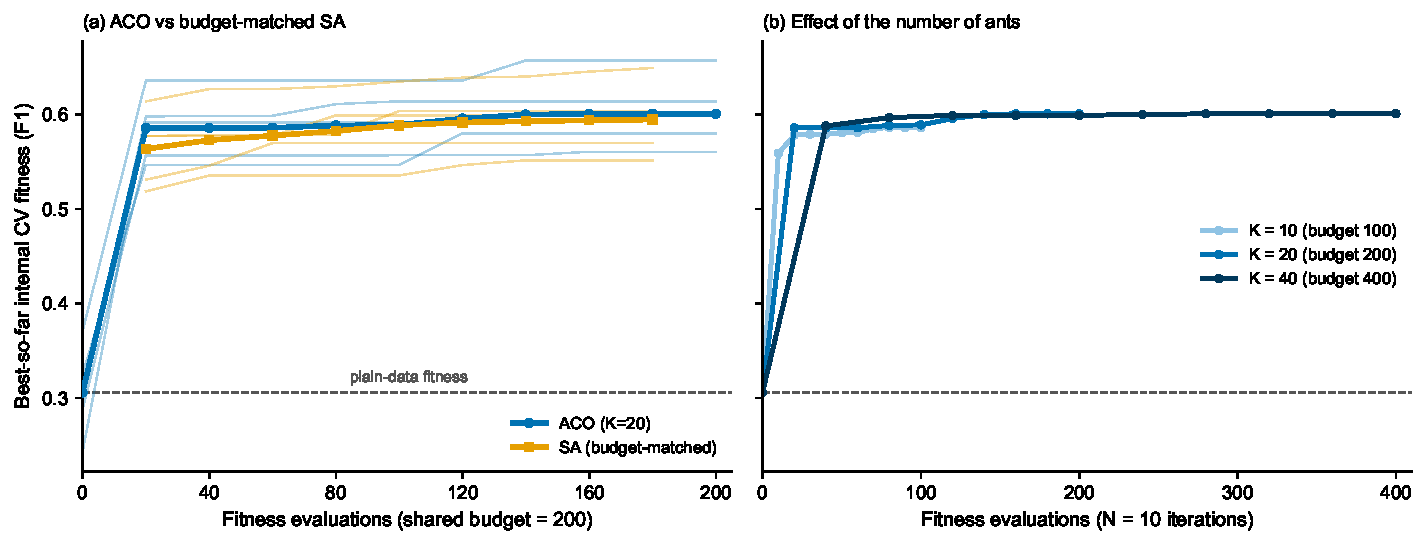
\includegraphics[width=\textwidth]{Fig3.pdf}
\caption{The convergence of the undersampling search on NR. (a) ACO
against the budget-matched SA, in which the thin lines denote individual
seeds. (b) ACO with $K \in \{10, 20, 40\}$ ants. The dashed line
denotes the plain-data fitness, i.e., the ACO abstention threshold}
\label{fig:convergence}
\end{figure}


\subsection{Interaction between the pool ratio and the selector}
\label{sec:ratio}
We next examined how the size of the synthetic pool interacts with the
type of selector. The six SHS-RUS and SHS-ACO variants were run on NR
with the three pool ratios, as summarized in Table~\ref{tab:ratio} and
illustrated in Figure~\ref{fig:ratio}. The two selectors show opposite
preferences. The best ratio of SHS-ACO is 1.5 for all three
oversamplers, i.e., the largest pool considered. In contrast, the best
ratio of SHS-RUS is 1.25 for the ROS and SMOTE arms and 1.0 for the
ADASYN arm, and its performance declines at the ratio of 1.5 in all
three arms.

This interaction can be explained by the role of the surplus
candidates. For an informed selector, a larger pool enlarges the choice
space, so that the search can exploit the surplus to find a better
subset. For a random selector, every candidate is equally likely to be
drawn, so that the surplus merely increases the chance of including
uninformative or noisy candidates. Therefore, the pool ratio is not a
property of the dataset alone but has to be chosen jointly with the
selector. This finding was used to set the per-arm ratios of the final
comparison described in Section~\ref{sec:design}.

\begin{table}[htbp]
\centering
\caption{The F1 scores of the SHS variants over the three pool ratios on NR (ten seeds for SHS-RUS and five for SHS-ACO), in which bold denotes the best ratio of each method.}
\label{tab:ratio}
\footnotesize
\begin{tabular}{lccc}
\toprule
Method & Ratio 1.00 & Ratio 1.25 & Ratio 1.50 \\
\midrule
SHS-RUS (ROS) & 0.4579 $\pm$ 0.0531 & \textbf{0.4725 $\pm$ 0.0611} & 0.4586 $\pm$ 0.0551 \\
SHS-RUS (SMOTE) & 0.3735 $\pm$ 0.0888 & \textbf{0.3759 $\pm$ 0.0856} & 0.3419 $\pm$ 0.0721 \\
SHS-RUS (ADASYN) & \textbf{0.3805 $\pm$ 0.0918} & 0.3665 $\pm$ 0.0899 & 0.3187 $\pm$ 0.0852 \\
SHS-ACO (ROS) & 0.4736 $\pm$ 0.0680 & 0.4390 $\pm$ 0.0518 & \textbf{0.4751 $\pm$ 0.0739} \\
SHS-ACO (SMOTE) & 0.3130 $\pm$ 0.0772 & 0.3381 $\pm$ 0.0675 & \textbf{0.3431 $\pm$ 0.0936} \\
SHS-ACO (ADASYN) & 0.3451 $\pm$ 0.0822 & 0.3276 $\pm$ 0.1264 & \textbf{0.3603 $\pm$ 0.1094} \\
\bottomrule
\end{tabular}
\end{table}

\begin{figure}[htbp]
\centering
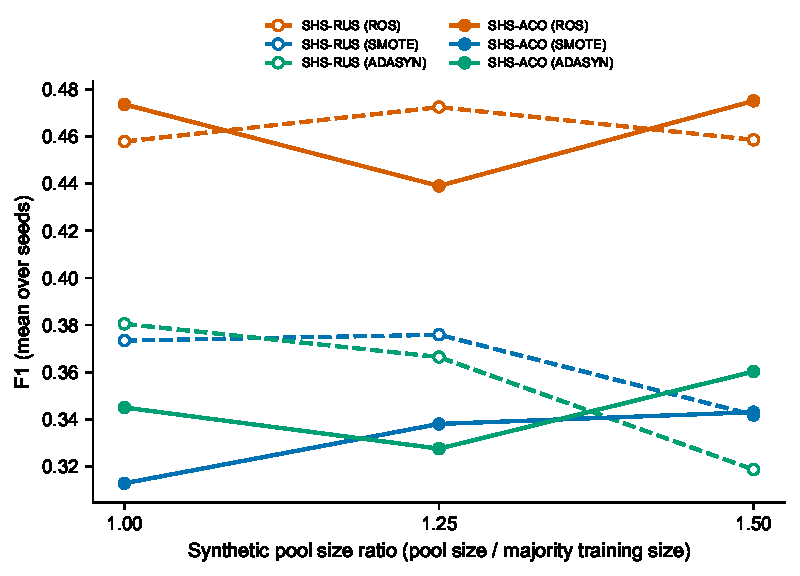
\includegraphics[width=0.75\textwidth]{Fig4.pdf}
\caption{The interaction between the pool ratio and the selector on NR}
\label{fig:ratio}
\end{figure}

\subsection{Main comparison across the four datasets}
\label{sec:main}
The main comparison of the 13 methods on the four datasets is summarized
in Table~\ref{tab:main}, and the per-dataset winners with their
statistical tests are given in Table~\ref{tab:tests}. The corresponding
G-Mean, balanced accuracy, and AUPRC
matrices are provided in Appendix~\ref{secA1}. Resampling pays
off substantially on three of the four datasets. On NR, the ROS family
dominates, in which SHS-RUS (ROS) reaches an F1 score of 0.4725 against
the baseline of 0.3235. On GPCR, the ROS family collapses to
approximately 0.24, while SHS-SA (SMOTE) leads with 0.3645, slightly
ahead of SMOTE-Tomek with 0.3614. On IC, SHS-ACO (ADASYN) leads with
0.3461 against the baseline of 0.1600. On Enzyme, no resampling method
beats the baseline of 0.1854, in which the closest competitors are the SHS-ACO variants with 0.1840, which equals the baseline mean over the same five seeds owing to the abstention described in
Section~\ref{sec:abstention}.

Two patterns emerge across the datasets. First, there is no universal
winner. The winning oversampler shifts from ROS on NR to SMOTE on GPCR,
ADASYN on IC, and no resampling on Enzyme, which follows the increasing
number of real positive training instances (63, 444, 1{,}033, and
2{,}048, respectively), as illustrated in Figure~\ref{fig:gradient}.
Second, the magnitude of the benefit does not decay gradually. The best
family keeps a margin of 0.15 to 0.19 F1 points over the baseline up to
IC and then collapses to zero or below on Enzyme.

The statistical tests support these observations. The winner differs
significantly from the baseline on NR ($p$ = 0.0059 over ten paired
seeds) and reaches the minimum attainable $p$ value of 0.0625 on GPCR
and IC with five paired seeds. In contrast, the winner is never
significantly different from the runner-up ($p \geq 0.43$), so that the
top of each dataset is occupied by a tight cluster of methods rather
than a single winner. Across the datasets, the Friedman test rejects the
equality of the 13 methods ($\chi^2$ = 42.5, $p$ = $2.7 \times
10^{-5}$ over 20 blocks). The best mean ranks belong to SHS-ACO (ADASYN)
with 4.85 and SHS-ACO (SMOTE) with 5.00, as shown in
Figure~\ref{fig:ranks}. However, the Nemenyi critical difference of
4.08 separates only the baseline, ROS, and SHS-RUS (ROS) from the
top-ranked method.

These results carry three messages. First, a winner identified on a
single split or a single dataset does not transfer, which confirms the
concern raised in Section~\ref{sec:seed} and underlines the need for repeated,
multi-dataset evaluation in this field. Second, the results suggest a
two-level explanation, in which the pairing between the oversampler and
the dataset sets the attainable performance ceiling, while the selector
only determines how closely that ceiling is approached. The increment of the
selection stage on top of the best plain oversampler shrinks
monotonically, i.e., $+0.015$ on NR, $+0.006$ on GPCR, and $+0.005$ on
IC, and turns into abstention on Enzyme. Notably, on NR this increment
is already achieved by the random selector. We hypothesize that the quality
of the synthetic candidates becomes more uniform when more real
positives are available, so that choosing among them adds little value.
Third, from a practical point of view, the oversampler should be matched
to the minority richness of the dataset, while an informed selector is
worth its cost only under extreme scarcity. If a single method must be
chosen blindly, SHS-ACO offers the best average rank together with a
built-in safety valve.

\begin{table}[htbp]
\centering
\caption{The F1 scores (mean $\pm$ SD) of the 13 methods on the four
datasets, in which bold denotes the best method of each dataset.}
\label{tab:main}
\setlength{\tabcolsep}{3pt}%
\footnotesize
\begin{tabular}{lccccc}
\toprule
Method & $n$ & NR & GPCR & IC & Enzyme \\
\midrule
Baseline & 10 & 0.3235 $\pm$ 0.0870 & 0.1925 $\pm$ 0.0388 & 0.1600 $\pm$ 0.0246 & \textbf{0.1854 $\pm$ 0.0158} \\
ROS & 10 & 0.4573 $\pm$ 0.0537 & 0.2404 $\pm$ 0.0098 & 0.2621 $\pm$ 0.0065 & 0.1137 $\pm$ 0.0019 \\
SMOTE & 10 & 0.3744 $\pm$ 0.0900 & 0.3582 $\pm$ 0.0371 & 0.3221 $\pm$ 0.0131 & 0.1726 $\pm$ 0.0067 \\
ADASYN & 10 & 0.3582 $\pm$ 0.1025 & 0.3098 $\pm$ 0.0405 & 0.3412 $\pm$ 0.0160 & 0.1489 $\pm$ 0.0049 \\
SMOTE-ENN & 10 & 0.3469 $\pm$ 0.0467 & 0.3184 $\pm$ 0.0216 & 0.3032 $\pm$ 0.0133 & 0.1726 $\pm$ 0.0076 \\
SMOTE-Tomek & 10 & 0.3890 $\pm$ 0.0815 & 0.3614 $\pm$ 0.0337 & 0.3203 $\pm$ 0.0139 & 0.1728 $\pm$ 0.0067 \\
SHS-RUS (ROS) & 10 & \textbf{0.4725 $\pm$ 0.0611} & 0.2393 $\pm$ 0.0090 & 0.2635 $\pm$ 0.0070 & 0.1137 $\pm$ 0.0026 \\
SHS-RUS (SMOTE) & 10 & 0.3759 $\pm$ 0.0856 & 0.3440 $\pm$ 0.0407 & 0.3206 $\pm$ 0.0144 & 0.1743 $\pm$ 0.0053 \\
SHS-RUS (ADASYN) & 10 & 0.3805 $\pm$ 0.0918 & 0.3199 $\pm$ 0.0417 & 0.3444 $\pm$ 0.0196 & 0.1512 $\pm$ 0.0047 \\
SHS-ACO (ROS) & 5 & 0.4338 $\pm$ 0.0619 & 0.2370 $\pm$ 0.0086 & 0.2684 $\pm$ 0.0080 & 0.1840 $\pm$ 0.0106 \\
SHS-ACO (SMOTE) & 5 & 0.3507 $\pm$ 0.1037 & 0.3516 $\pm$ 0.0596 & 0.3246 $\pm$ 0.0184 & 0.1840 $\pm$ 0.0106 \\
SHS-ACO (ADASYN) & 5 & 0.3930 $\pm$ 0.0889 & 0.2890 $\pm$ 0.0519 & \textbf{0.3461 $\pm$ 0.0224} & 0.1840 $\pm$ 0.0106 \\
SHS-SA (SMOTE) & 5 & 0.3467 $\pm$ 0.0738 & \textbf{0.3645 $\pm$ 0.0554} & 0.3205 $\pm$ 0.0148 & 0.1707 $\pm$ 0.0034 \\
\bottomrule
\end{tabular}
\end{table}

\begin{table}[htbp]
\centering
\caption{The best methods per dataset with the paired Wilcoxon
signed-rank tests on F1.}
\label{tab:tests}
\setlength{\tabcolsep}{2pt}%
\footnotesize
\begin{tabular}{lcccccc}
\toprule
Dataset & Best method & F1 & Runner-up & $p$ (runner-up) & F1 baseline & $p$ (baseline) \\
\midrule
NR & SHS-RUS (ROS) & 0.4725 & ROS & 0.8203 & 0.3235 & 0.0059 \\
GPCR & SHS-SA (SMOTE) & 0.3645 & SMOTE-Tomek & 0.6250 & 0.1925 & 0.0625 \\
IC & SHS-ACO (ADASYN) & 0.3461 & SHS-RUS (ADASYN) & 0.4375 & 0.1600 & 0.0625 \\
Enzyme & Baseline & 0.1854 & SHS-ACO (ADASYN) & -- & 0.1854 & -- \\
\bottomrule
\end{tabular}
\end{table}

\begin{figure}[htbp]
\centering
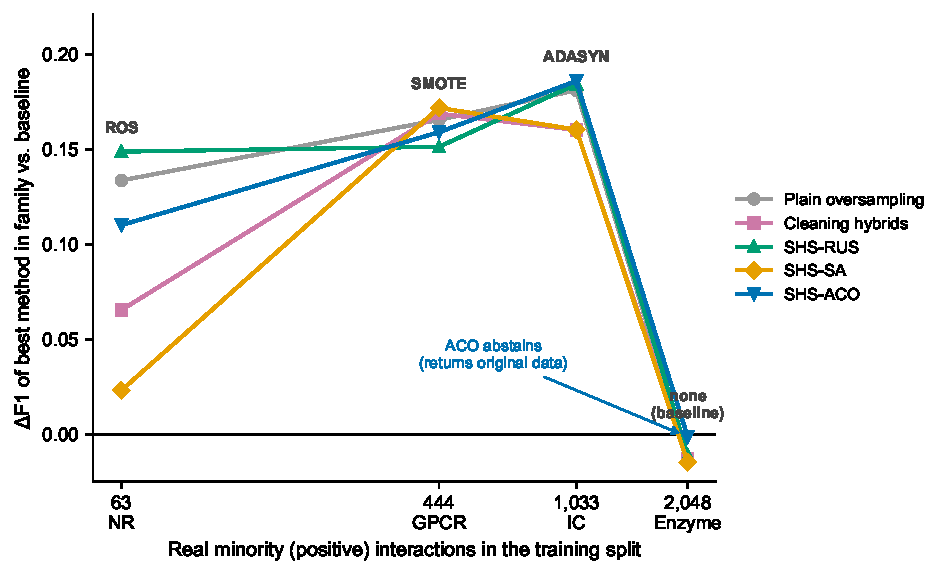
\includegraphics[width=0.9\textwidth]{Fig5.pdf}
\caption{The gain of the best method in each family over the baseline
across the four datasets, ordered by the number of real positive
training instances}
\label{fig:gradient}
\end{figure}

\begin{figure}[htbp]
\centering
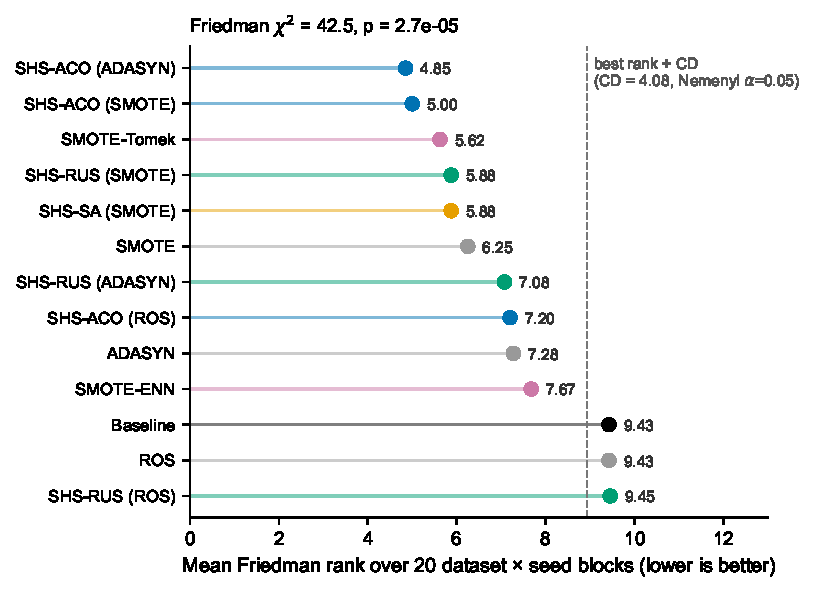
\includegraphics[width=0.8\textwidth]{Fig6.pdf}
\caption{The mean Friedman ranks of the 13 methods with the Nemenyi
critical difference}
\label{fig:ranks}
\end{figure}

\subsection{Abstention property of the ACO undersampler}
\label{sec:abstention}
On Enzyme, the abstention mechanism described in
Section~\ref{sec:aco} was triggered in every run. In all 15 ACO runs on
this dataset, i.e., the three oversampler arms with five seeds each,
the search never found a synthetic subset whose internal fitness
exceeded that of the unmodified training data, so that the
undersampler returned the original training data. We verified this behavior on the test side,
in which the confusion matrices of all 15 runs are identical to those of
the baseline, as summarized in Table~\ref{tab:abstention}.

The contrast with SA is instructive. SA has no abstention action and
always returns a balanced training set, so that it was forced to add
synthetic candidates on Enzyme. Its mean F1 score of 0.1707 lies below the baseline mean of 0.1840 over the same five seeds, and below the per-seed baseline in four of the
five seeds. The gap is not statistically significant at five seeds
($p$ = 0.125), yet the direction is consistent.

This behavior shows that informed selection equipped with a null action
doubles as a safety valve. When resampling is harmful, a selector that
may decline to resample converts a potential loss into a no-operation,
while a selector without this option inherits the harm. We therefore
recommend the abstention action as an explicit design element for
optimization-based resampling methods.

\begin{table}[htbp]
\centering
\caption{The verification of the ACO abstention on Enzyme, in which
identical denotes a confusion matrix equal to that of the baseline.}
\label{tab:abstention}
\footnotesize
\begin{tabular}{lccccc}
\toprule
Seed & F1 baseline & ACO (ROS) & ACO (SMOTE) & ACO (ADASYN) & F1 SHS-SA (SMOTE) \\
\midrule
0 & 0.1889 & identical & identical & identical & 0.1684 \\
1 & 0.1711 & identical & identical & identical & 0.1716 \\
2 & 0.1980 & identical & identical & identical & 0.1690 \\
3 & 0.1860 & identical & identical & identical & 0.1762 \\
4 & 0.1761 & identical & identical & identical & 0.1682 \\
\bottomrule
\end{tabular}
\end{table}

\subsection{Comparison between ACO and SA}
The direct comparison between ACO and SA on the SMOTE arm is summarized
in Table~\ref{tab:savsaco}. The difference is not significant on any
dataset ($p$ between 0.125 and 0.8125 over five paired seeds). SA leads
nominally on GPCR (0.3645 against 0.3516), while ACO leads nominally on
NR, IC, and Enzyme, in which the Enzyme gap of $+0.0133$ stems entirely
from the abstention described in Section~\ref{sec:abstention}.

The internal view of the search is consistent with the external one.
Under the matched budget, both searches improve rapidly within the first
20 evaluations and then flatten, reaching nearly identical final fitness
values of 0.601 for ACO and 0.595 for SA
(Figure~\ref{fig:convergence}a). Neither search is starved by the
budget, so that the equivalence cannot be attributed to an unfinished
search.

These results answer the question of why ACO should be preferred over
other metaheuristics. In terms of search quality, it should not be,
since a budget-matched SA \citep{kirkpatrick1983optimization,
chennuru2022simulated} is statistically indistinguishable. The value of
SHS therefore lies in informed selection itself rather than in a
particular metaheuristic, and a practitioner may choose the simpler or
more familiar optimizer. The distinguishing feature is the abstention
action rather than the search strategy, and any metaheuristic equipped
with the same null action would likely inherit this advantage.

\begin{table}[htbp]
\centering
\caption{The budget-matched comparison between SHS-ACO (SMOTE) and
SHS-SA (SMOTE) on the four datasets.}
\label{tab:savsaco}
\footnotesize
\begin{tabular}{lccccc}
\toprule
Dataset & F1 SHS-ACO (SMOTE) & F1 SHS-SA (SMOTE) & Diff. & $n$ & $p$ (Wilcoxon) \\
\midrule
NR & 0.3507 & 0.3467 & +0.0039 & 5 & 0.8125 \\
GPCR & 0.3516 & 0.3645 & -0.0128 & 5 & 0.3750 \\
IC & 0.3246 & 0.3205 & +0.0042 & 5 & 0.6250 \\
Enzyme & 0.1840 & 0.1707 & +0.0133 & 5 & 0.1250 \\
\bottomrule
\end{tabular}
\end{table}

\subsection{Computational cost}
The runtime per seed is summarized in Table~\ref{tab:runtime}. The
uninformed methods are cheap, in which the classical oversamplers, the
hybrids, and the SHS-RUS variants complete within seconds to a few
minutes and stay within a factor of six of the baseline. The informed
selectors are in a different class. ACO and SA require from 22 minutes
per seed on NR up to approximately 52 hours per seed on IC, i.e., two to
three orders of magnitude above the cheap methods, with a factor of up to approximately 1,930 relative to the baseline. The factors on Enzyme are smaller
(between 52 and 60) because the baseline itself is expensive on this
dataset and the search uses the faster HistGB fitness with only $N = 5$ iterations. The cost of SA
equals that of ACO by construction, while halving the number of ants to
$K = 10$ halves the cost without a measurable quality loss
(Section~\ref{sec:ablation}).

This cost has to be weighed against the gain. On GPCR and IC, the
increments of the best informed arm over the best plain oversampler are
$+0.006$ and $+0.005$ F1 at a cost of 17 and 43 hours per seed, respectively. On NR,
the cheap SHS-RUS variant already exceeds the informed arms, and on
Enzyme the honest outcome of a multi-hour search is to change nothing.
Therefore, informed selection is justified mainly when the dataset is
small enough that its absolute cost stays within minutes to an hour,
which coincides with the extreme-scarcity regime where selection matters
most. For larger datasets, a well-chosen plain oversampler delivers
nearly the same performance at a negligible cost.

\begin{table}[htbp]
\centering
\caption{The mean runtime per seed of the 13 methods, in which the
factor in parentheses denotes the ratio to the baseline of the same
dataset.}
\label{tab:runtime}
\footnotesize
\begin{tabular}{lrrrr}
\toprule
Method & NR & GPCR & IC & Enzyme \\
\midrule
Baseline (no resampling) & 2.1\,s (1$\times$) & 39.1\,s (1$\times$) & 1.6\,min (1$\times$) & 13.0\,min (1$\times$) \\
ROS & 3.4\,s (2$\times$) & 1.2\,min (2$\times$) & 2.9\,min (2$\times$) & 25.0\,min (2$\times$) \\
SMOTE & 7.6\,s (4$\times$) & 2.2\,min (3$\times$) & 6.8\,min (4$\times$) & 1.0\,h (5$\times$) \\
ADASYN & 7.1\,s (3$\times$) & 2.1\,min (3$\times$) & 6.2\,min (4$\times$) & 57.0\,min (4$\times$) \\
SMOTE-ENN & 7.3\,s (3$\times$) & 2.5\,min (4$\times$) & 8.3\,min (5$\times$) & 1.2\,h (6$\times$) \\
SMOTE-Tomek & 7.7\,s (4$\times$) & 2.6\,min (4$\times$) & 8.5\,min (5$\times$) & 1.2\,h (5$\times$) \\
SHS-RUS (ROS) & 3.5\,s (2$\times$) & 1.2\,min (2$\times$) & 2.9\,min (2$\times$) & 25.2\,min (2$\times$) \\
SHS-RUS (SMOTE) & 7.8\,s (4$\times$) & 2.2\,min (3$\times$) & 6.9\,min (4$\times$) & 1.0\,h (5$\times$) \\
SHS-RUS (ADASYN) & 6.9\,s (3$\times$) & 2.1\,min (3$\times$) & 6.2\,min (4$\times$) & 58.8\,min (5$\times$) \\
SHS-ACO (ROS) & 22.5\,min (635$\times$) & 8.6\,h (790$\times$) & 20.8\,h (779$\times$) & 11.2\,h (52$\times$) \\
SHS-ACO (SMOTE) & 49.4\,min (1394$\times$) & 15.4\,h (1419$\times$) & 45.1\,h (1691$\times$) & 12.1\,h (56$\times$) \\
SHS-ACO (ADASYN) & 48.2\,min (1360$\times$) & 13.3\,h (1225$\times$) & 43.2\,h (1621$\times$) & 12.3\,h (57$\times$) \\
SHS-SA (SMOTE) & 58.0\,min (1634$\times$) & 17.2\,h (1583$\times$) & 51.5\,h (1930$\times$) & 12.9\,h (60$\times$) \\
\bottomrule
\end{tabular}
\end{table}

% =========================================================================
\subsection{Limitations and future work}
Several limitations qualify these findings. First, the unlabeled pairs
were treated as negatives, so that some true interactions may be
mislabeled. This assumption is shared by most studies on these datasets,
but it may compress the measurable differences between methods. Second,
the expensive arms were run with five seeds, which limits the
statistical power, in which the minimum attainable Wilcoxon $p$ value is
0.0625. The consistent directions of the differences across datasets
partly compensate for this limit. Third, the internal fitness on Enzyme
used HistGB instead of GB for feasibility. The substitution was uniform
within the dataset, yet it may interact with the abstention behavior.
Fourth, all conclusions rest on a single classifier and a single domain,
so that the gradient observed here should be confirmed beyond GB and
beyond DTI data.

These limitations suggest several directions. The evaluation can be
extended to other classifiers and to imbalanced domains outside DTI to
test the generality of the minority-richness gradient. The main obstacle
of informed selection is its cost, so that a cheap surrogate fitness,
e.g., a subsampled or lower-fidelity estimate, is an attractive
direction. Finally, other metaheuristics such as genetic algorithms or
particle swarm optimization can be equipped with the same abstention
action, which we expect to matter more than the choice of the search
strategy itself.

% =========================================================================
\section{Conclusions}
This study evaluated the sequential hybrid sampling framework with
informed undersampling on four DTI datasets under a repeated and
statistically tested protocol of 725 runs. The framework is valid but
conditional. On the smallest and most positive-scarce dataset,
resampling lifts the best F1 score from 0.32 to 0.47 and the selection
stage adds a further increment, while on the larger datasets a
well-chosen plain oversampler is nearly optimal, and on the richest
dataset the best action is not to resample at all, in which no method
beats the baseline F1 score of 0.19 and the ACO undersampler discovers
this by itself through its abstention action in all 15 runs. The winning
oversampler shifts from ROS to SMOTE and ADASYN along the growing number
of real positives, so that the oversampler should be matched to the
minority richness of the dataset, and the SHS-ACO variants offer the
safest blind choice with the best mean Friedman ranks of 4.85 and 5.00
among the 13 methods. The choice of the metaheuristic is secondary, in
which a budget-matched SA performs on par with ACO ($p \geq 0.125$ on
every dataset), while the abstention action is the design element worth
keeping. Informed selection costs up to about 460 times more than random selection, so that it pays off mainly under extreme
scarcity. We also showed that a single-split evaluation can reorder the
methods by chance alone, in which the F1 score of one configuration
varied from 0.27 to 0.43 across the splits. We therefore recommend
repeated multi-seed evaluation with paired statistical tests as the
standard protocol for resampling studies in DTI prediction. All code,
data pipelines, and results are publicly available to support
reproduction and extension.

\section*{Declarations}

\bmhead{Funding}
% TODO: konfirmasi — pernyataan tanpa pendanaan:
No funding was received to assist with the preparation of this
manuscript.

\bmhead{Competing interests}
The authors have no competing interests to declare that are relevant to
the content of this article.

\bmhead{Data and code availability}
The source code, the data preparation pipeline, all result files, and
the scripts that regenerate every table and figure of this article are
available at \url{https://github.com/ismankrn/aco-shs} (release v1.0.1). An archived snapshot of the repository is deposited on Zenodo
(DOI \href{https://doi.org/10.5281/zenodo.23686130}%
{10.5281/zenodo.23686130}). The feature
matrices can be regenerated from the SRX-DTI source data by using the
included scripts \citep{khojasteh2023improving}.

\bmhead{Author contributions}
Isman Kurniawan contributed to the conceptualization, methodology,
validation, investigation, resources, visualization, and supervision of
the study, and to the writing of the original draft and the review and
editing of the manuscript. Rizky Nurhaliza Harahap contributed to the
methodology, validation, investigation, and resources, and to the
review and editing of the manuscript. Fhira Nhita contributed to the supervision of the study and to the review
and editing of the manuscript. Afizan Azman contributed to the
validation of the study and to the review and editing of the
manuscript. All authors read and approved the final manuscript.

\begin{appendices}

\section{Additional evaluation metrics}\label{secA1}

Tables~\ref{tab:sgmean}--\ref{tab:sauprc} complement the main comparison in
Table~\ref{tab:main} with the remaining three evaluation metrics. Each cell
gives the mean $\pm$ standard deviation over the seeds, and bold denotes
the best method of each dataset.

\begin{table}[htbp]
\centering
\caption{The G-Mean scores (mean $\pm$ SD) of the 13 methods on the four datasets.}
\label{tab:sgmean}
\setlength{\tabcolsep}{3pt}%
\footnotesize
\begin{tabular}{lccccc}
\toprule
Method & $n$ & NR & GPCR & IC & Enzyme \\
\midrule
Baseline & 10 & 0.4709 $\pm$ 0.0754 & 0.3332 $\pm$ 0.0386 & 0.3004 $\pm$ 0.0260 & 0.3272 $\pm$ 0.0149 \\
ROS & 10 & 0.7296 $\pm$ 0.0490 & 0.7925 $\pm$ 0.0131 & 0.8265 $\pm$ 0.0076 & \textbf{0.8456 $\pm$ 0.0071} \\
SMOTE & 10 & 0.5498 $\pm$ 0.0733 & 0.5511 $\pm$ 0.0367 & 0.6519 $\pm$ 0.0121 & 0.6554 $\pm$ 0.0150 \\
ADASYN & 10 & 0.5438 $\pm$ 0.0855 & 0.5054 $\pm$ 0.0404 & 0.6560 $\pm$ 0.0164 & 0.6402 $\pm$ 0.0119 \\
SMOTE-ENN & 10 & 0.6364 $\pm$ 0.0525 & 0.6879 $\pm$ 0.0212 & 0.7080 $\pm$ 0.0143 & 0.6612 $\pm$ 0.0217 \\
SMOTE-Tomek & 10 & 0.5609 $\pm$ 0.0632 & 0.5527 $\pm$ 0.0343 & 0.6473 $\pm$ 0.0148 & 0.6551 $\pm$ 0.0150 \\
SHS-RUS (ROS) & 10 & \textbf{0.7358 $\pm$ 0.0503} & \textbf{0.7933 $\pm$ 0.0141} & 0.8286 $\pm$ 0.0085 & 0.8449 $\pm$ 0.0081 \\
SHS-RUS (SMOTE) & 10 & 0.5442 $\pm$ 0.0693 & 0.5314 $\pm$ 0.0359 & 0.6451 $\pm$ 0.0122 & 0.6579 $\pm$ 0.0138 \\
SHS-RUS (ADASYN) & 10 & 0.5621 $\pm$ 0.0720 & 0.5130 $\pm$ 0.0415 & 0.6561 $\pm$ 0.0201 & 0.6449 $\pm$ 0.0158 \\
SHS-ACO (ROS) & 5 & 0.7134 $\pm$ 0.0581 & 0.7898 $\pm$ 0.0100 & \textbf{0.8296 $\pm$ 0.0096} & 0.3260 $\pm$ 0.0095 \\
SHS-ACO (SMOTE) & 5 & 0.5382 $\pm$ 0.0820 & 0.5478 $\pm$ 0.0575 & 0.6525 $\pm$ 0.0210 & 0.3260 $\pm$ 0.0095 \\
SHS-ACO (ADASYN) & 5 & 0.5837 $\pm$ 0.0729 & 0.4872 $\pm$ 0.0541 & 0.6684 $\pm$ 0.0196 & 0.3260 $\pm$ 0.0095 \\
SHS-SA (SMOTE) & 5 & 0.5344 $\pm$ 0.0548 & 0.5581 $\pm$ 0.0576 & 0.6458 $\pm$ 0.0165 & 0.6474 $\pm$ 0.0059 \\
\bottomrule
\end{tabular}
\end{table}

\begin{table}[htbp]
\centering
\caption{The balanced accuracy scores (mean $\pm$ SD) of the 13 methods on the four datasets.}
\label{tab:sbas}
\setlength{\tabcolsep}{3pt}%
\footnotesize
\begin{tabular}{lccccc}
\toprule
Method & $n$ & NR & GPCR & IC & Enzyme \\
\midrule
Baseline & 10 & 0.6087 $\pm$ 0.0359 & 0.5555 $\pm$ 0.0124 & 0.5447 $\pm$ 0.0079 & 0.5534 $\pm$ 0.0048 \\
ROS & 10 & 0.7537 $\pm$ 0.0390 & 0.7957 $\pm$ 0.0120 & 0.8267 $\pm$ 0.0075 & \textbf{0.8461 $\pm$ 0.0069} \\
SMOTE & 10 & 0.6449 $\pm$ 0.0424 & 0.6481 $\pm$ 0.0203 & 0.6995 $\pm$ 0.0084 & 0.7046 $\pm$ 0.0100 \\
ADASYN & 10 & 0.6413 $\pm$ 0.0498 & 0.6237 $\pm$ 0.0208 & 0.7036 $\pm$ 0.0110 & 0.6926 $\pm$ 0.0079 \\
SMOTE-ENN & 10 & 0.6829 $\pm$ 0.0365 & 0.7241 $\pm$ 0.0155 & 0.7341 $\pm$ 0.0111 & 0.7084 $\pm$ 0.0144 \\
SMOTE-Tomek & 10 & 0.6509 $\pm$ 0.0379 & 0.6490 $\pm$ 0.0189 & 0.6965 $\pm$ 0.0101 & 0.7044 $\pm$ 0.0101 \\
SHS-RUS (ROS) & 10 & \textbf{0.7591 $\pm$ 0.0401} & \textbf{0.7964 $\pm$ 0.0126} & 0.8288 $\pm$ 0.0082 & 0.8454 $\pm$ 0.0078 \\
SHS-RUS (SMOTE) & 10 & 0.6423 $\pm$ 0.0401 & 0.6376 $\pm$ 0.0193 & 0.6952 $\pm$ 0.0085 & 0.7063 $\pm$ 0.0092 \\
SHS-RUS (ADASYN) & 10 & 0.6510 $\pm$ 0.0425 & 0.6278 $\pm$ 0.0210 & 0.7040 $\pm$ 0.0135 & 0.6958 $\pm$ 0.0105 \\
SHS-ACO (ROS) & 5 & 0.7407 $\pm$ 0.0450 & 0.7930 $\pm$ 0.0093 & \textbf{0.8299 $\pm$ 0.0094} & 0.5529 $\pm$ 0.0031 \\
SHS-ACO (SMOTE) & 5 & 0.6369 $\pm$ 0.0491 & 0.6468 $\pm$ 0.0316 & 0.7001 $\pm$ 0.0145 & 0.5529 $\pm$ 0.0031 \\
SHS-ACO (ADASYN) & 5 & 0.6626 $\pm$ 0.0479 & 0.6148 $\pm$ 0.0268 & 0.7118 $\pm$ 0.0140 & 0.5529 $\pm$ 0.0031 \\
SHS-SA (SMOTE) & 5 & 0.6337 $\pm$ 0.0320 & 0.6527 $\pm$ 0.0312 & 0.6957 $\pm$ 0.0112 & 0.6992 $\pm$ 0.0036 \\
\bottomrule
\end{tabular}
\end{table}

\begin{table}[htbp]
\centering
\caption{The AUPRC values (mean $\pm$ SD) of the 13 methods on the four datasets.}
\label{tab:sauprc}
\setlength{\tabcolsep}{3pt}%
\footnotesize
\begin{tabular}{lccccc}
\toprule
Method & $n$ & NR & GPCR & IC & Enzyme \\
\midrule
Baseline & 10 & 0.4015 $\pm$ 0.0816 & \textbf{0.3439 $\pm$ 0.0300} & \textbf{0.4081 $\pm$ 0.0337} & \textbf{0.3191 $\pm$ 0.0131} \\
ROS & 10 & 0.4038 $\pm$ 0.0720 & 0.3091 $\pm$ 0.0323 & 0.3636 $\pm$ 0.0289 & 0.1643 $\pm$ 0.0092 \\
SMOTE & 10 & 0.3665 $\pm$ 0.0816 & 0.3241 $\pm$ 0.0333 & 0.2663 $\pm$ 0.0307 & 0.0958 $\pm$ 0.0055 \\
ADASYN & 10 & 0.3400 $\pm$ 0.0625 & 0.2829 $\pm$ 0.0261 & 0.2511 $\pm$ 0.0235 & 0.0816 $\pm$ 0.0035 \\
SMOTE-ENN & 10 & 0.2739 $\pm$ 0.0505 & 0.2884 $\pm$ 0.0272 & 0.2513 $\pm$ 0.0188 & 0.0967 $\pm$ 0.0066 \\
SMOTE-Tomek & 10 & 0.3645 $\pm$ 0.0847 & 0.3242 $\pm$ 0.0327 & 0.2638 $\pm$ 0.0271 & 0.0960 $\pm$ 0.0056 \\
SHS-RUS (ROS) & 10 & \textbf{0.4240 $\pm$ 0.0734} & 0.3121 $\pm$ 0.0260 & 0.3617 $\pm$ 0.0289 & 0.1634 $\pm$ 0.0077 \\
SHS-RUS (SMOTE) & 10 & 0.3612 $\pm$ 0.0861 & 0.3158 $\pm$ 0.0290 & 0.2597 $\pm$ 0.0243 & 0.0966 $\pm$ 0.0042 \\
SHS-RUS (ADASYN) & 10 & 0.3557 $\pm$ 0.0636 & 0.2801 $\pm$ 0.0257 & 0.2533 $\pm$ 0.0241 & 0.0837 $\pm$ 0.0034 \\
SHS-ACO (ROS) & 5 & 0.3763 $\pm$ 0.0565 & 0.2935 $\pm$ 0.0358 & 0.3779 $\pm$ 0.0218 & 0.3188 $\pm$ 0.0185 \\
SHS-ACO (SMOTE) & 5 & 0.3326 $\pm$ 0.0677 & 0.3104 $\pm$ 0.0425 & 0.2708 $\pm$ 0.0256 & 0.3188 $\pm$ 0.0185 \\
SHS-ACO (ADASYN) & 5 & 0.3209 $\pm$ 0.0551 & 0.2800 $\pm$ 0.0352 & 0.2609 $\pm$ 0.0234 & 0.3188 $\pm$ 0.0185 \\
SHS-SA (SMOTE) & 5 & 0.3436 $\pm$ 0.0850 & 0.3204 $\pm$ 0.0391 & 0.2735 $\pm$ 0.0214 & 0.0954 $\pm$ 0.0027 \\
\bottomrule
\end{tabular}
\end{table}

\end{appendices}

\bibliography{references}

\end{document}
